\documentclass[preprint,12pt]{elsarticle}

\usepackage{amsmath,amssymb,amsfonts,amsthm,bm,mathtools}
\usepackage{booktabs,multirow,array,threeparttable}
\usepackage{graphicx}
\usepackage{caption}
\usepackage{float}
\usepackage{siunitx}
\usepackage{hyperref}
\usepackage{enumitem}
\usepackage{tikz}
\usepackage{url}
\usetikzlibrary{arrows.meta,positioning,shapes.geometric}

\journal{Control Engineering Practice}
\graphicspath{
  {figures/}
  {../code/project_method3c_lccznn_solver/results/method2_scheme_b_positive_dlccznn/live/}
  {../code/project_method3c_lccznn_solver/results/method2_scheme_b_positive_dlccznn/offline/}
  {../code/project_method3c_lccznn_solver/results/method3c_position_and_drift_lccznn/live/}
  {../code/project_method3a_pcg_solver/results/method3a_position_and_drift_pcg/live/}
}
\hypersetup{colorlinks=true,linkcolor=blue,citecolor=blue,urlcolor=blue}
\sisetup{
  detect-all,
  scientific-notation = true,
  round-mode = places,
  round-precision = 3
}

\newtheorem{proposition}{Proposition}
\newtheorem{remark}{Remark}

\newcommand{\R}{\mathbb{R}}
\newcommand{\q}{\bm{q}}
\newcommand{\qd}{\dot{\bm{q}}}
\newcommand{\ep}{\bm{e}_{\mathrm{p}}}
\newcommand{\ed}{\bm{e}_{\mathrm{d}}}
\newcommand{\x}{\bm{x}}
\newcommand{\xd}{\bm{x}_{\mathrm{d}}}
\newcommand{\rd}{\dot{\bm{r}}_{\mathrm{d}}}
\newcommand{\J}{\bm{J}}
\newcommand{\methodone}{Method~1}
\newcommand{\methodtwo}{Method~2}
\newcommand{\methodthree}{Method~3a}
\newcommand{\methodoneDL}{Method~1~DLCCZNN}
\newcommand{\methodtwoDL}{Method~2~DLCCZNN}
\newcommand{\methodthreepcg}{Method~3a~PCG}
\newcommand{\methodthreelcc}{Method~3c~LCCZNN}

\begin{document}

\begin{frontmatter}

\title{Sampled DLCCZNN realization of a classic drift free kinematic resolution formulation for redundant manipulators}

\author[1]{Yuxuan Li}
\author[1]{Junpei Yang}
\author[1]{Zhan Li\corref{cor1}}
\cortext[cor1]{Corresponding author.}
\ead{zhan.li@swjtu.edu.cn}
\address[1]{School of Mechanical Engineering, Southwest Jiaotong University, Chengdu 611756, China}

\begin{abstract}
Classic drift free repetitive motion planning of redundant manipulators is well established, yet its derivation and solver interpretation remain largely rooted in continuous time neural dynamics. Real robot controllers, however, operate in sampled form and can spend only a finite computational budget within each control period. The primary contribution of this paper is a formulation preserving sampled \methodtwoDL{} controller for the classic drift free kinematic resolution problem. The method starts from the strongest classical formulation preserving baseline and tracks the Karush Kuhn Tucker residual through projected DLCCZNN dynamics with matrix vector products, scalar residual shaping, and explicit velocity box projection. To position this contribution precisely, the paper separates two design questions that are often mixed together in the literature: improvement by objective reformulation and improvement by solver redesign under a fixed formulation. The baseline comparison identifies \methodtwo{} as the strongest formulation preserving anchor and \methodthree{} as a high accuracy reference obtained by changing the sampled objective itself. A discrete time analysis then establishes local residual contraction, sampled outer loop tracking bounds, and a residual to command mismatch relation for the proposed controller. Offline UR3e tests over a \SI{20}{\second} cycle and simulator based real time control loop validation in CoppeliaSim over a \SI{10}{\second} cycle show that the proposed \methodtwoDL{} reduces the mean position error of the classical \methodtwo{} from \SI{3.686e-4}{\meter} to \SI{2.466e-4}{\meter} and its final joint drift norm from \SI{4.551e-3}{\radian} to \SI{1.430e-3}{\radian}. A dedicated parameter study further shows that the offline optimum and the real time optimum do not coincide, so the retained setting must be selected according to cycle end drift recovery rather than idealized replay accuracy alone. Auxiliary studies clarify the role of tight algorithmic and structural coupling: \methodthreepcg{} remains strong on the rewritten Method~3 objective, whereas a direct LCCZNN transfer to that objective loses drift recovery despite small instantaneous position error. These results support \methodtwoDL{} as the main route for carrying the classic drift free formulation into sampled robot control.
\end{abstract}

\begin{keyword}
redundant manipulators \sep repetitive motion control \sep drift free control \sep low computational complexity zeroing neural network \sep quadratic programming \sep sampled data control
\end{keyword}

\end{frontmatter}

\section{Introduction}

Redundant manipulators can exploit extra degrees of freedom for tracking, posture regulation, joint limit avoidance, and singularity avoidance. In repetitive tasks, however, redundancy also creates the classical joint drift problem: the end effector may return to a periodic Cartesian path while the joints fail to recover the initial posture at the end of each cycle. Once this cycle end error accumulates, the manipulator can gradually lose manipulability or move toward joint limits. For this reason, drift free repetitive motion planning remains a representative benchmark problem in robot kinematic control \citep{zhang2009rmp,zhang2017three}.

The classical route is to formulate repetitive inverse kinematics as a constrained quadratic program and to solve it online by recurrent neural dynamics \citep{wang2004recurrent,toshani2014ik,tan2022physical,hassan2020review}. In the drift free setting of \citet{zhang2009rmp}, the objective combines posture recovery, task equality, and dynamic velocity bounds converted from joint limits. This formulation is elegant and still influential, but its derivation and solver interpretation come mainly from a continuous time neural dynamics viewpoint. In practice, industrial and simulator based robot control is executed in sampled form, with explicit control periods, finite inner iterations, and communication induced mismatch. The sampled controller therefore needs a discrete interpretation rather than a direct inheritance from continuous time analysis.

LCCZNN and DLCCZNN offer an appealing route because they replace dense matrix inversion by residual driven iterative dynamics and preserve a clear error system interpretation \citep{zheng2024lccznn,qiu2022jerk,yang2025predefined,wen2024firstsecond,li2026dlccznn}. Yet the present comparative study also shows that direct solver replacement is not automatically beneficial. Some replacements preserve the drift free closed loop property, whereas others produce small instantaneous position errors but destroy cycle end posture recovery. This indicates that the real control issue is not only numerical efficiency, but tight coupling between algorithmic dynamics and control structure under a finite sampling budget.

The paper is built around a question that is easy to state but often blurred in existing work: when moving from continuous time drift free planning to sampled robot control, should one change the objective, change the solver, or do both? This paper answers that question in a deliberate order. The original \methodone{}, \methodtwo{}, and \methodthree{} are first retained as baseline formulations. Among them, \methodthree{} reaches the highest raw accuracy because it changes the objective itself, whereas \methodtwo{} is the strongest baseline that still preserves the classic drift free kinematic resolution formulation. This makes \methodtwo{} the right anchor for the main contribution of the paper: a sampled \methodtwoDL{} solver derived directly from the code level implementation and interpreted in control terms. To avoid an overly narrow story, three auxiliary lines are also retained: \methodoneDL{} as a weaker formulation preserving transfer, \methodthreelcc{} as a direct LCCZNN replacement of the Method~3 objective, and \methodthreepcg{} as a secondary structured solver for the Method~3 discrete subproblem.

The main contributions are as follows.
\begin{itemize}[leftmargin=1.5em]
  \item A formulation preserving sampled \methodtwoDL{} controller is proposed for the classic drift free kinematic resolution problem. Starting from the strongest classical formulation preserving baseline, its update law tracks the sampled Karush Kuhn Tucker residual by projected DLCCZNN dynamics, so the solver remains close to the logic of sampled robot control rather than continuous time transcription.
  \item A discrete control interpretation is established for the classical drift free repetitive motion quadratic program and for the proposed controller, including the explicit role of task feedback velocity, one step error propagation, dynamic velocity bounds induced by physical limits, and the sampled residual to command mismatch relation.
  \item A unified comparison is built across the original baseline methods and the auxiliary solver variants \methodoneDL{}, \methodthreelcc{}, and \methodthreepcg{}. This comparison reveals which gains come from formulation preserving solver design and which gains come from changing the optimization objective itself, thereby giving the paper a clear scientific hierarchy instead of a flat list of methods.
  \item Offline UR3e simulations and simulator based real time control loop validation in CoppeliaSim show that the proposed \methodtwoDL{} improves the classical \methodtwo{} under sampled execution, while the auxiliary comparisons clarify both the promise and the limits of alternative solver transfers. The parameter study further shows that offline and real time optima do not coincide, so drift recovery under sampled execution must guide the final retained setting.
\end{itemize}

The remainder of the paper is organized as follows. Section~2 reviews drift free repetitive motion planning and low complexity neural solvers. Section~3 formulates the discrete control problem. Section~4 presents the baseline methods, the proposed \methodtwoDL{}, and the auxiliary solver variants. Section~5 analyzes the proposed solver. Sections~6 and 7 report the experimental design and results. Section~8 concludes the paper.

\section{Related work}

\subsection{Drift free repetitive motion planning}

Drift free repetitive motion planning was developed to resolve the conflict between end effector periodicity and joint posture recovery in redundant manipulators. The representative formulation of \citet{zhang2009rmp} introduced a drift suppression term together with task equality and dynamic velocity bounds converted from joint limits, which yielded a compact online quadratic program. Later studies compared several recurrent neural solvers under the same repetitive motion planning formulation and showed that solver dynamics can substantially affect numerical behavior even when the outer optimization model is unchanged \citep{zhang2017three}. This classical line remains the control foundation of the present work.

\subsection{Neural dynamic solvers for constrained inverse kinematics}

Recurrent neural networks have long been used as online solvers for redundant manipulator inverse kinematics and constrained quadratic programming \citep{wang2004recurrent,toshani2014ik}. More recent work has continued this direction for physical constraints, Lyapunov analysis, and real time execution \citep{tan2022physical}. A broad review is given in \citet{hassan2020review}. These contributions establish the practical importance of neural dynamic optimization, but they do not resolve the sampled drift free control issue considered here, namely how the solver design should interact with the discrete repetitive motion objective.

\subsection{LCCZNN, DLCCZNN, and sampled robot control}

LCCZNN has been shown to reduce the computational burden of solving dynamic nonlinear equations while preserving a residual driven structure that is convenient for control oriented interpretation \citep{zheng2024lccznn}. Follow up studies extended this line to time varying quadratic programming and robot kinematic control \citep{yang2025predefined,wen2024firstsecond,yang2026enhanced}. Discrete ZNN models further demonstrated that sampled implementation should be treated as a first class design problem rather than a mere discretization afterthought \citep{qiu2022jerk}. Our recent DLCCZNN study reaches the same conclusion for UR3e trajectory tracking \citep{li2026dlccznn}. The current paper continues this sampled control viewpoint, but applies it to the drift free repetitive motion problem.

\subsection{Positioning of this paper}

The novelty of this paper lies in control level positioning rather than in proposing a universal new ZNN theory. The main scientific question is which solver reformulation is most suitable when drift free repetitive inverse kinematics must run in sampled form. The paper therefore distinguishes three cases that are often conflated in the literature: preserving the classic drift free kinematic resolution formulation and changing only the solver, changing the outer discrete objective itself, and transferring a low complexity solver into an objective whose closed loop meaning is not preserved by that transfer. This distinction is what motivates the choice of \methodtwoDL{} as the main method and the use of \methodthreepcg{} only as a secondary comparison.

\section{Problem formulation}

\subsection{Manipulator kinematics and drift definition}

Consider a redundant manipulator with joint vector $\q_k \in \R^n$ at sampling instant $k$ and end effector position
\begin{equation}
  \x(\q_k) = f(\q_k) \in \R^m,
\end{equation}
where $n > m$. Let the desired Cartesian trajectory be $\xd(k)$ with desired task velocity $\rd(k)$. We define the position tracking error and joint drift error as
\begin{equation}
  \ep(k) = \x(\q_k) - \xd(k),
\end{equation}
\begin{equation}
  \ed(k) = \q_k - \q_0,
\end{equation}
where $\q_0$ is the initial joint posture at the beginning of the repetitive task.

The drift free requirement concerns the cycle end residual rather than the transient joint excursion. During the task, the joints are allowed to move substantially. What matters is whether the final posture returns close to $\q_0$ after one completed cycle.

The sampled control architecture studied in this paper is summarized in Fig.~\ref{fig:sampled_architecture}. This figure is useful because it makes the central design choice explicit: the proposed method retains the classic drift free kinematic resolution formulation and modifies the sampled solver layer, rather than replacing the entire control objective.

\begin{figure}[t]
  \centering
  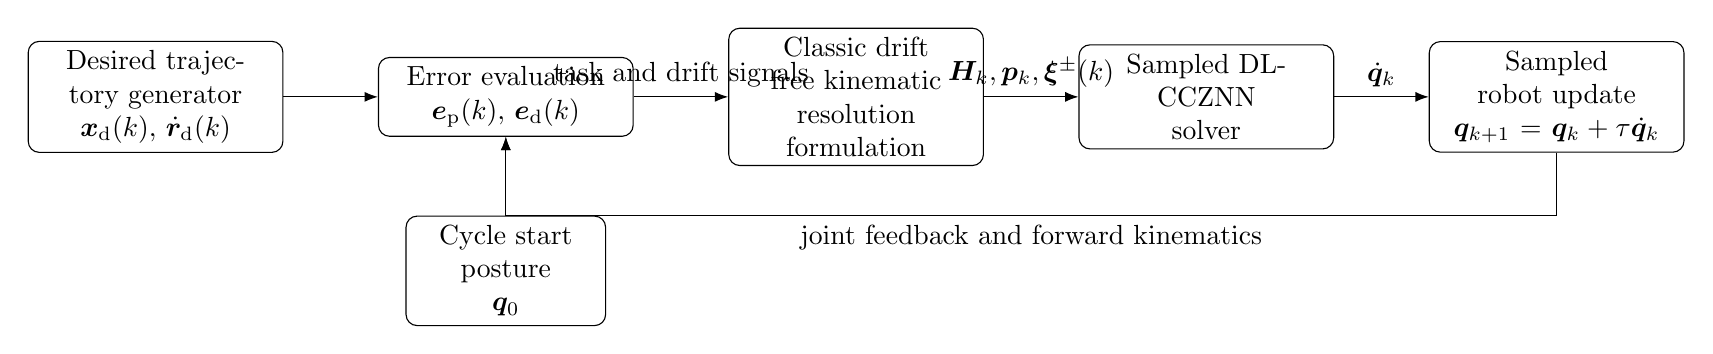
\begin{tikzpicture}[
    node distance=10mm and 12mm,
    >=Latex,
    block/.style={draw, rounded corners, align=center, minimum height=9mm, text width=30mm},
    smallblock/.style={draw, rounded corners, align=center, minimum height=8mm, text width=23mm}
  ]
    \node[block] (traj) {Desired trajectory generator\\$\xd(k),\,\rd(k)$};
    \node[block, right=of traj] (error) {Error evaluation\\$\ep(k),\,\ed(k)$};
    \node[smallblock, below=of error] (q0) {Cycle start posture\\$\q_0$};
    \node[block, right=of error] (scheme) {Classic drift free kinematic\\resolution formulation};
    \node[block, right=of scheme] (solver) {Sampled DLCCZNN\\solver};
    \node[block, right=of solver] (plant) {Sampled robot update\\$\q_{k+1}=\q_k+\tau\qd_k$};

    \draw[->] (traj) -- (error);
    \draw[->] (q0) -- (error);
    \draw[->] (error) -- node[above]{task and drift signals} (scheme);
    \draw[->] (scheme) -- node[above]{$\bm{H}_k,\bm{p}_k,\bm{\xi}^{\pm}(k)$} (solver);
    \draw[->] (solver) -- node[above]{$\qd_k$} (plant);
    \draw[->] (plant.south) |- ++(0,-0.8) -| node[pos=0.25, below]{joint feedback and forward kinematics} (error.south);
  \end{tikzpicture}
  \caption{Sampled control architecture of the studied system. The proposed method keeps the classic drift free kinematic resolution formulation and changes the sampled solver layer.}
  \label{fig:sampled_architecture}
\end{figure}

\subsection{One step sampled model}

Let $\tau > 0$ be the outer control period. A first order linearization around $\q_k$ gives
\begin{equation}
  \x(\q_{k+1}) \approx \x(\q_k) + \tau \J_k \qd_k,
  \label{eq:fk_linearization}
\end{equation}
where $\J_k = \J(\q_k)$ is the task Jacobian and $\qd_k$ is the joint velocity command at step $k$. The joint update is
\begin{equation}
  \q_{k+1} = \q_k + \tau \qd_k.
  \label{eq:joint_update}
\end{equation}

If the desired trajectory is discretized by
\begin{equation}
  \xd(k+1) \approx \xd(k) + \tau \rd(k),
\end{equation}
then the one step position error satisfies
\begin{equation}
  \ep(k+1) \approx \ep(k) + \tau \bigl(\J_k \qd_k - \rd(k)\bigr),
  \label{eq:ep_basic}
\end{equation}
and the joint drift error propagates as
\begin{equation}
  \ed(k+1) = \ed(k) + \tau \qd_k.
  \label{eq:ed_basic}
\end{equation}

\subsection{Why the task equality uses feedback velocity}

The classic drift free kinematic resolution formulation does not impose $\J_k \qd_k = \rd(k)$ directly. Instead, it uses the feedback corrected velocity
\begin{equation}
  \bm{b}_{\mathrm{fb}}(k) = \rd(k) - k_{\mathrm{p}} \ep(k),
  \label{eq:bfb}
\end{equation}
with task gain $k_{\mathrm{p}} > 0$. The reason is immediate from \eqref{eq:ep_basic}. If $\J_k \qd_k = \rd(k)$, then $\ep(k+1) \approx \ep(k)$, so the existing task error is simply carried forward. If one enforces
\begin{equation}
  \J_k \qd_k = \rd(k) - k_{\mathrm{p}} \ep(k),
  \label{eq:task_feedback_constraint}
\end{equation}
then
\begin{equation}
  \ep(k+1) \approx (1 - \tau k_{\mathrm{p}})\ep(k),
\end{equation}
which makes the sampled position correction explicit. This is why the classical drift free formulations use task feedback velocity rather than pure task velocity.

\subsection{Dynamic velocity bounds}

Let the joint position and velocity bounds be
\begin{equation}
  \bm{\theta}_{\min} \le \q_k \le \bm{\theta}_{\max},
\end{equation}
\begin{equation}
  \dot{\bm{\theta}}_{\min} \le \qd_k \le \dot{\bm{\theta}}_{\max}.
\end{equation}
Following \citet{zhang2009rmp}, the position limits are converted into dynamic velocity limits:
\begin{equation}
  \bm{\xi}^{-}(k) =
  \max\!\left(
    \dot{\bm{\theta}}_{\min},
    \frac{\eta}{\tau}\left( \bm{\theta}_{\min} - \q_k \right)
  \right),
\end{equation}
\begin{equation}
  \bm{\xi}^{+}(k) =
  \min\!\left(
    \dot{\bm{\theta}}_{\max},
    \frac{\eta}{\tau}\left( \bm{\theta}_{\max} - \q_k \right)
  \right),
\end{equation}
where $\eta \in (0,1]$ is a safety factor. These bounds guarantee that the next step update \eqref{eq:joint_update} remains feasible.

\subsection{Classic formulation and discrete objective}

The equality constrained formulation shared by \methodone{} and \methodtwo{} is
\begin{equation}
  \begin{aligned}
    \min_{\qd_k} \quad &
      \frac{1}{2}\qd_k^\top \bm{W}\qd_k + \hat{\bm{c}}(k)^\top \qd_k \\
    \text{s.t.} \quad &
      \J_k \qd_k = \bm{b}_{\mathrm{fb}}(k), \\
    &
      \bm{\xi}^{-}(k) \le \qd_k \le \bm{\xi}^{+}(k),
  \end{aligned}
  \label{eq:classical_qp_shell}
\end{equation}
where $\bm{W}$ is positive definite and $\hat{\bm{c}}(k)$ biases the solution toward drift recovery.

By contrast, \methodthree{} is built directly from the one step predictions \eqref{eq:ep_basic} and \eqref{eq:ed_basic}. With positive weights $\alpha$ and $\beta$, the sampled objective is
\begin{equation}
  \begin{aligned}
    \min_{\qd_k} \quad &
      \alpha
      \left\|
        \ep(k) + \tau\bigl(\J_k\qd_k - \rd(k) + k_{\mathrm{p}}\ep(k)\bigr)
      \right\|_2^2 \\
      & \quad +
      \beta
      \left\|
        \ed(k) + \tau \qd_k
      \right\|_2^2 \\
    \text{s.t.} \quad &
      \bm{\xi}^{-}(k) \le \qd_k \le \bm{\xi}^{+}(k).
  \end{aligned}
  \label{eq:method3_original}
\end{equation}

The methods studied in this paper are therefore divided into three families.
\begin{itemize}[leftmargin=1.5em]
  \item \methodone{}, \methodtwo{}, \methodoneDL{}, and \methodtwoDL{} preserve the classic equality constrained formulation in \eqref{eq:classical_qp_shell}.
  \item \methodthree{} and \methodthreepcg{} use the discrete sampled objective in \eqref{eq:method3_original}.
  \item \methodthreelcc{} keeps the Method~3 outer objective but replaces its inner linear solve by an LCCZNN style residual tracker.
\end{itemize}

This separation is central to the later discussion because it distinguishes solver improvement from objective reformulation.

\section{Classic formulations and the proposed sampled DLCCZNN controller}

\subsection{Original baseline formulations}

\methodone{} and \methodtwo{} both start from the classic drift free kinematic resolution formulation \eqref{eq:classical_qp_shell}. In the integrated scripts used in this work, $\bm{W}$ is the identity matrix and the drift bias is constructed from the cycle deviation:
\begin{equation}
  \hat{\bm{c}}(k) = \mu_{\mathrm{a}} \, \psi\!\bigl(\ed(k)\bigr),
\end{equation}
where $\mu_{\mathrm{a}} > 0$ and the elementwise activation is
\begin{equation}
  \psi_i(z_i)
  =
  \operatorname{sign}(z_i)\,|z_i|^{\rho_{\mathrm{a}}}
  \exp\!\bigl(\min(|z_i|,c_{\mathrm{a}})\bigr).
  \label{eq:drift_activation}
\end{equation}
The difference between \methodone{} and \methodtwo{} lies mainly in the inner primal dual dynamics. \methodone{} uses a simplified projected primal dual update, whereas \methodtwo{} introduces a positive residual energy shaping term. Because \methodtwo{} will later be shown to be the strongest baseline that still preserves the classic formulation, it is selected as the anchor for the proposed solver.

\methodthree{} changes the problem layer rather than the solver layer. Define
\begin{equation}
  \bm{a}_k
  =
  \left( \frac{1}{\tau} + k_{\mathrm{p}} \right)\ep(k) - \rd(k).
  \label{eq:ak}
\end{equation}
Ignoring constants that do not affect the optimizer, \eqref{eq:method3_original} becomes
\begin{equation}
  \begin{aligned}
    \min_{\qd_k} \quad &
      \frac{1}{2}\qd_k^\top \bm{Q}_k \qd_k + \bm{c}_k^\top \qd_k \\
    \text{s.t.} \quad &
      \bm{\xi}^{-}(k) \le \qd_k \le \bm{\xi}^{+}(k),
  \end{aligned}
  \label{eq:method3_qp}
\end{equation}
with
\begin{equation}
  \bm{Q}_k = \alpha \J_k^\top \J_k + \beta \bm{I} + \varepsilon \bm{I},
  \label{eq:method3_Q}
\end{equation}
\begin{equation}
  \bm{c}_k
  =
  \alpha \J_k^\top \bm{a}_k
  +
  \beta \frac{\ed(k)}{\tau}.
  \label{eq:method3_c}
\end{equation}
This sampled objective is useful as a high accuracy reference, but it no longer answers the formulation preserving question that is central to the proposed method.

\subsection{Proposed \methodtwoDL{}}

Starting from the \methodtwo{} formulation, define the optimization problem
\begin{equation}
  \begin{aligned}
    \min_{\qd_k} \quad &
      \frac{1}{2}\qd_k^\top \qd_k + \hat{\bm{c}}_2(k)^\top \qd_k \\
    \text{s.t.} \quad &
      \J_k \qd_k = \bm{b}_{\mathrm{fb}}(k), \\
    &
      \bm{\xi}^{-}(k) \le \qd_k \le \bm{\xi}^{+}(k),
  \end{aligned}
  \label{eq:method2_shell}
\end{equation}
with
\begin{equation}
  \hat{\bm{c}}_2(k) = \mu_{\mathrm{a}} \, \psi\!\bigl(\ed(k)\bigr).
\end{equation}

For the equality constrained part of \eqref{eq:method2_shell}, introduce the primal dual vector
\begin{equation}
  \bm{y}_\ell =
  \begin{bmatrix}
    \qd_\ell \\
    \bm{\lambda}_\ell
  \end{bmatrix}
  \in \R^{n+m},
\end{equation}
and define
\begin{equation}
  \bm{H}_k =
  \begin{bmatrix}
    \bm{I} & -\J_k^\top \\
    \J_k & \bm{0}
  \end{bmatrix},
  \qquad
  \bm{p}_k =
  \begin{bmatrix}
    \hat{\bm{c}}_2(k) \\
    -\bm{b}_{\mathrm{fb}}(k)
  \end{bmatrix}.
  \label{eq:method2_Hp}
\end{equation}
The sampled KKT residual is
\begin{equation}
  \bm{r}_\ell = \bm{H}_k \bm{y}_\ell + \bm{p}_k,
  \qquad
  v_\ell = \frac{1}{2}\|\bm{r}_\ell\|_2^2.
  \label{eq:method2_residual}
\end{equation}

At each outer control step, $\bm{H}_k$ and $\bm{p}_k$ are frozen and the inner DLCCZNN tracker runs for at most $N_s$ substeps with inner step size $h = \tau / N_s$. Let
\begin{equation}
  \phi(v_\ell)
  =
  v_\ell^{\rho_{\mathrm{s}}}
  \exp\!\bigl(\min(v_\ell,c_{\mathrm{s}})\bigr),
  \qquad
  0 < \rho_{\mathrm{s}} < 1,
  \label{eq:method2_phi}
\end{equation}
and define the normalized residual direction
\begin{equation}
  \bm{d}_\ell
  =
  \frac{\bm{H}_k^\top \bm{r}_\ell}
  {\|\bm{H}_k^\top \bm{r}_\ell\|_2^2 + \lambda_{\mathrm{s}}},
  \label{eq:method2_direction}
\end{equation}
where $\lambda_{\mathrm{s}} > 0$ avoids singular normalization. The raw DLCCZNN update is
\begin{equation}
  \bm{y}_{\ell+1}^{\mathrm{raw}}
  =
  \bm{y}_\ell
  -
  h \gamma_{\mathrm{s}} \phi(v_\ell)\bm{d}_\ell.
  \label{eq:method2_raw_update}
\end{equation}
Only the primal part is projected onto the dynamic velocity box:
\begin{equation}
  \qd_{\ell+1}
  =
  \Pi_{[\bm{\xi}^{-}(k),\bm{\xi}^{+}(k)]}
  \bigl([\bm{y}_{\ell+1}^{\mathrm{raw}}]_{1:n}\bigr),
  \label{eq:method2_primal_proj}
\end{equation}
\begin{equation}
  \bm{\lambda}_{\ell+1}
  =
  [\bm{y}_{\ell+1}^{\mathrm{raw}}]_{n+1:n+m},
\end{equation}
which gives
\begin{equation}
  \bm{y}_{\ell+1}
  =
  \begin{bmatrix}
    \qd_{\ell+1} \\
    \bm{\lambda}_{\ell+1}
  \end{bmatrix}.
  \label{eq:method2_final_update}
\end{equation}
The applied joint command at control step $k$ is the final primal part $\qd_k = \qd_{N_s}$.

The control meaning of \methodtwoDL{} is therefore explicit. The solver is not treated as a continuous time neural dynamics running in the background. Instead, the code level sampled implementation is itself the design object: the outer drift free formulation generates $\bm{H}_k$ and $\bm{p}_k$, and the inner residual tracker spends a prescribed number of operations to reduce the KKT inconsistency before the control period ends. This interpretation is practically important because the controller never waits for asymptotic neural convergence; it can only spend a fixed amount of work inside each sample.

\subsection{Auxiliary solver variants}

Three auxiliary variants are retained only to delimit the main contribution. \methodoneDL{} applies the same sampled residual tracking logic to the weaker \methodone{} formulation and therefore tests whether solver replacement alone can compensate for a weaker outer design. \methodthreelcc{} starts from the Method~3 quadratic form \eqref{eq:method3_qp} and rewrites its optimality condition as
\begin{equation}
  \bm{Q}_k \qd_k + \bm{c}_k = \bm{0}.
\end{equation}
An LCCZNN style residual tracker is then applied to this linear root problem. \methodthreepcg{} keeps the same sampled objective \eqref{eq:method3_qp}, but solves the corresponding linear system by a warm started projected conjugate gradient iteration with a fixed iteration cap. These two variants are not developed as parallel protagonists. They are kept only to separate the effects of formulation strength, sampled solver structure, and objective rewriting in Section~7.

\section{Discrete time analysis of the proposed method}

The analysis in this section is carried out in the standard sampled data local regime relevant to the implemented controller. During one outer control period, $\bm{H}_k$ and $\bm{p}_k$ are frozen. The task Jacobian is assumed to remain bounded and locally full row rank. For clarity, the main derivations are written for the interior regime where the box projection is inactive; when a fixed active set is present, the same arguments apply on the corresponding reduced coordinates provided that the reduced KKT matrix remains nonsingular.

\subsection{KKT consistency inside the classic formulation}

\begin{proposition}
Assume that $\J_k$ has full row rank and that no component of the optimizer hits the box bounds at control step $k$. Then any vector $\bm{y}_k^\star = [\qd_k^{\star\top},\bm{\lambda}_k^{\star\top}]^\top$ satisfying
\begin{equation}
  \bm{H}_k \bm{y}_k^\star + \bm{p}_k = \bm{0}
  \label{eq:kkt_zero}
\end{equation}
is the unique solution of the equality constrained problem \eqref{eq:method2_shell} without active box constraints.
\end{proposition}

\begin{proof}
Equation \eqref{eq:kkt_zero} expands into
\begin{equation}
  \qd_k^\star - \J_k^\top \bm{\lambda}_k^\star + \hat{\bm{c}}_2(k) = \bm{0},
\end{equation}
\begin{equation}
  \J_k \qd_k^\star - \bm{b}_{\mathrm{fb}}(k) = \bm{0}.
\end{equation}
These are exactly the stationarity and equality feasibility conditions of \eqref{eq:method2_shell}. The quadratic term has Hessian equal to the identity matrix, hence the objective is strictly convex in $\qd_k$. Because $\J_k$ has full row rank, the equality constraints are regular. Therefore the equality constrained problem has a unique optimizer, and $\qd_k^\star$ is that optimizer.
\end{proof}

The proposition clarifies what the inner residual tracker is solving. It is not an arbitrary neural state equation; it is a sampled approximation of the KKT root of the classic drift free formulation. When box constraints become active, the final control signal is obtained by the explicit projection \eqref{eq:method2_primal_proj}, so feasibility is preserved even though the equality constrained root is no longer the applied command exactly.

\subsection{Discrete time residual contraction in the local interior regime}

\begin{proposition}
Define
\begin{equation}
  \bm{r}_\ell = \bm{H}_k \bm{y}_\ell + \bm{p}_k,
\end{equation}
\begin{equation}
  \bm{g}_\ell = \bm{H}_k^\top \bm{r}_\ell,
\end{equation}
\begin{equation}
  V_\ell = \frac{1}{2}\|\bm{r}_\ell\|_2^2,
\end{equation}
and the effective scalar step size
\begin{equation}
  \eta_\ell
  =
  \frac{h\gamma_{\mathrm{s}}\phi(V_\ell)}
  {\|\bm{g}_\ell\|_2^2 + \lambda_{\mathrm{s}}}.
  \label{eq:eta_ell}
\end{equation}
Assume that the primal box projection is inactive at inner step $\ell$, so the update becomes
\begin{equation}
  \bm{y}_{\ell+1} = \bm{y}_\ell - \eta_\ell \bm{g}_\ell.
  \label{eq:inner_unprojected}
\end{equation}
Then
\begin{equation}
  V_{\ell+1} - V_\ell
  \le
  -
  \left(
    \eta_\ell - \frac{\|\bm{H}_k\|_2^2}{2}\eta_\ell^2
  \right)
  \|\bm{g}_\ell\|_2^2.
  \label{eq:V_contract}
\end{equation}
Consequently, if
\begin{equation}
  0 < \eta_\ell < \frac{2}{\|\bm{H}_k\|_2^2},
  \label{eq:eta_cond}
\end{equation}
then $V_{\ell+1} < V_\ell$ whenever $\bm{g}_\ell \neq \bm{0}$.
\end{proposition}

\begin{proof}
From \eqref{eq:inner_unprojected},
\begin{equation}
  \bm{r}_{\ell+1}
  =
  \bm{H}_k(\bm{y}_\ell - \eta_\ell \bm{g}_\ell) + \bm{p}_k
  =
  \bm{r}_\ell - \eta_\ell \bm{H}_k \bm{g}_\ell.
\end{equation}
Therefore
\begin{equation}
  V_{\ell+1} - V_\ell
  =
  -\eta_\ell \bm{r}_\ell^\top \bm{H}_k \bm{g}_\ell
  + \frac{\eta_\ell^2}{2}\|\bm{H}_k \bm{g}_\ell\|_2^2.
\end{equation}
Since $\bm{g}_\ell = \bm{H}_k^\top \bm{r}_\ell$, the first term is
\begin{equation}
  \bm{r}_\ell^\top \bm{H}_k \bm{g}_\ell
  =
  \bm{g}_\ell^\top \bm{g}_\ell
  =
  \|\bm{g}_\ell\|_2^2.
\end{equation}
Moreover,
\begin{equation}
  \|\bm{H}_k \bm{g}_\ell\|_2
  \le
  \|\bm{H}_k\|_2 \|\bm{g}_\ell\|_2.
\end{equation}
Substituting these two relations into the previous equation gives \eqref{eq:V_contract}. If \eqref{eq:eta_cond} holds, then the coefficient multiplying $\|\bm{g}_\ell\|_2^2$ is strictly positive, and thus $V_{\ell+1} < V_\ell$ whenever $\bm{g}_\ell \neq \bm{0}$.
\end{proof}

The proposition gives the discrete time Lyapunov inequality that is missing in a purely continuous time narrative. In the implemented controller, the primal part is projected onto the admissible box. This projection is nonexpansive and keeps the applied velocity feasible. Hence the sampled update remains bounded globally, whereas the strict contraction law above governs each interior segment, and each fixed active set segment can be analyzed through the corresponding reduced system.

\subsection{Sampled outer loop tracking bound}

\begin{proposition}
Let $\qd_k^\star$ denote the interior optimizer of \eqref{eq:method2_shell} and define the solver mismatch
\begin{equation}
  \bm{s}_k = \qd_k - \qd_k^\star.
\end{equation}
Assume $\|\J_k\|_2 \le \bar J$ for all $k$, and let the first order linearization remainder in \eqref{eq:fk_linearization} satisfy
\begin{equation}
  \|\bm{\delta}_k\|_2 \le c_{\mathrm{x}}\tau^2.
\end{equation}
Then the position tracking error of the sampled outer loop satisfies
\begin{equation}
  \ep(k+1)
  =
  (1-\tau k_{\mathrm{p}})\ep(k)
  +
  \tau \J_k \bm{s}_k
  +
  \bm{\delta}_k.
  \label{eq:ep_ss}
\end{equation}
If $0 < \tau k_{\mathrm{p}} < 2$ and $\|\bm{s}_k\|_2 \le \bar s$, then
\begin{equation}
  \|\ep(k)\|_2
  \le
  \rho^k \|\ep(0)\|_2
  +
  \frac{\tau \bar J \bar s + c_{\mathrm{x}}\tau^2}{1-\rho},
  \qquad
  \rho = |1-\tau k_{\mathrm{p}}|,
  \label{eq:ep_bound}
\end{equation}
and therefore
\begin{equation}
  \limsup_{k\to\infty}\|\ep(k)\|_2
  =
  \mathcal{O}(\bar s + \tau).
\end{equation}
\end{proposition}

\begin{proof}
The ideal interior optimizer satisfies
\begin{equation}
  \J_k \qd_k^\star = \rd(k) - k_{\mathrm{p}}\ep(k).
\end{equation}
Substituting $\qd_k = \qd_k^\star + \bm{s}_k$ into the one step prediction \eqref{eq:ep_basic} gives
\begin{equation}
  \ep(k+1)
  =
  \ep(k)
  + \tau\bigl(\J_k \qd_k^\star - \rd(k)\bigr)
  + \tau \J_k \bm{s}_k
  + \bm{\delta}_k,
\end{equation}
which leads to \eqref{eq:ep_ss}. Taking norms yields
\begin{equation}
  \|\ep(k+1)\|_2
  \le
  \rho \|\ep(k)\|_2
  +
  \tau \bar J \bar s
  +
  c_{\mathrm{x}}\tau^2.
\end{equation}
Standard iteration of this scalar inequality gives \eqref{eq:ep_bound}.
\end{proof}

The proposition provides the outer loop meaning of the inner residual suppression. It shows that sampled tracking performance is controlled by two terms: the discretization remainder $\mathcal{O}(\tau)$ and the solver mismatch level $\bar s$. Therefore a solver that lowers the residual more effectively inside each sample directly tightens the sampled tracking bound.

\subsection{Residual to command mismatch relation}

\begin{proposition}
Assume that $\J_k$ has full row rank in the operating region of interest and that the smallest singular value of $\bm{H}_k$ is bounded below by a positive constant $\underline{\sigma}_{\mathrm{H}}$. Then
\begin{equation}
  \|\bm{s}_k\|_2
  \le
  \underline{\sigma}_{\mathrm{H}}^{-1}
  \|\bm{r}_{N_s}(k)\|_2.
  \label{eq:residual_to_command}
\end{equation}
\end{proposition}

\begin{proof}
Let $\bm{y}_k^\star$ be the interior KKT solution at control step $k$. Since
\begin{equation}
  \bm{r}_{N_s}(k)
  =
  \bm{H}_k\bigl(\bm{y}_{N_s}(k)-\bm{y}_k^\star\bigr),
\end{equation}
and $\bm{H}_k$ is nonsingular in the local operating region, one has
\begin{equation}
  \bm{y}_{N_s}(k)-\bm{y}_k^\star
  =
  \bm{H}_k^{-1}\bm{r}_{N_s}(k).
\end{equation}
Therefore
\begin{equation}
  \|\bm{y}_{N_s}(k)-\bm{y}_k^\star\|_2
  \le
  \|\bm{H}_k^{-1}\|_2 \|\bm{r}_{N_s}(k)\|_2
  \le
  \underline{\sigma}_{\mathrm{H}}^{-1}\|\bm{r}_{N_s}(k)\|_2.
\end{equation}
Taking the primal part gives \eqref{eq:residual_to_command}.
\end{proof}

Combining \eqref{eq:ep_bound} and \eqref{eq:residual_to_command} shows why the residual plot is not a cosmetic diagnostic. It is a control relevant quantity that bounds the command mismatch and therefore affects sampled tracking accuracy. The final cycle drift is likewise sensitive to this mismatch because
\begin{equation}
  \ed(N)
  =
  \ed(0)
  +
  \tau \sum_{k=0}^{N-1}\qd_k^\star
  +
  \tau \sum_{k=0}^{N-1}\bm{s}_k.
\end{equation}
The classic formulation shapes the first sum, whereas the sampled solver quality determines the size of the second sum.

\subsection{Per sample computational cost}

For fixed $N_s$, each inner substep of \methodtwoDL{} requires one multiplication by $\bm{H}_k$, one multiplication by $\bm{H}_k^\top$, one scalar activation, and one projection of the primal part onto the velocity box. Since $\bm{H}_k \in \R^{(n+m)\times(n+m)}$, the dominant per sample cost is
\begin{equation}
  \mathcal{O}\!\bigl(N_s(n+m)^2\bigr).
  \label{eq:method2_complexity}
\end{equation}

For \methodthreepcg{}, forming $\bm{Q}_k$ from $\J_k \in \R^{m\times n}$ costs $\mathcal{O}(mn^2)$, and $k$ conjugate gradient iterations cost $\mathcal{O}(kn^2)$. Hence
\begin{equation}
  \mathcal{O}\!\bigl((m+k)n^2\bigr)
\end{equation}
per sample, where $k$ is the realized number of inner iterations.

In the present UR3e problem, $n=6$ and $m=3$, so both costs are small in absolute terms. The main merit of \methodtwoDL{} is therefore not a dramatic wall clock advantage on a tiny system. Its value lies in preserving the classic formulation, maintaining an explicit sampled control interpretation, and avoiding dense direct matrix inversion within the formulation preserving line.

\subsection{Design implication for this paper}

The baseline data later show that \methodthree{} reaches the best raw accuracy because it directly optimizes the sampled one step tracking and drift objective. That result is important, but it answers a different design question. The main question of the present paper is whether the classic drift free kinematic resolution formulation itself can be made more suitable for sampled robot control through a DLCCZNN inspired solver. From this viewpoint, \methodtwoDL{} is the principal route: it starts from the strongest formulation preserving baseline, admits a discrete time residual analysis, and retains drift recovery in closed loop. The auxiliary comparisons are kept precisely to make this claim rigorous rather than rhetorical.

\section{Experimental setup}

\subsection{Platform and task}

All experiments use a six degree of freedom UR3e manipulator model. The Cartesian task is a heart shaped trajectory in the $YZ$ plane with scale factor $0.008$. The trajectory is translated so that its initial point coincides with the end effector position generated by
\begin{equation}
  \q_0 =
  \begin{bmatrix}
    0 & -\pi/2 & \pi/2 & 0 & \pi/2 & 0
  \end{bmatrix}^{\top},
\end{equation}
which removes artificial startup mismatch in the offline studies.

Two execution modes are used at the current stage of the study.
\begin{itemize}[leftmargin=1.5em]
  \item \textbf{Offline mode:} numerical replay over a full \SI{20}{\second} cycle with the same kinematic model in controller and plant.
  \item \textbf{Real time control loop validation:} synchronous CoppeliaSim execution through the remote API. The main real time comparison uses \SI{10}{\second} cycles. An additional \SI{20}{\second} run of the original \methodthree{} is available as an auxiliary long period reference.
\end{itemize}

\subsection{Compared methods}

The compared methods are organized into three groups.
\begin{itemize}[leftmargin=1.5em]
  \item \textbf{Original baselines:} \methodone{}, \methodtwo{}, and \methodthree{}.
  \item \textbf{Formulation preserving solver transfers:} \methodoneDL{}, the default \methodtwoDL{}, and the tuned proposed \methodtwoDL{}.
  \item \textbf{Auxiliary structure matching studies:} \methodthreelcc{} and \methodthreepcg{}.
\end{itemize}

The purpose of the first group is to identify the baseline control structure. The second group tests whether the classic formulation can be improved through sampled DLCCZNN design. The third group explains why good raw numerical performance does not automatically make a method the main contribution of this paper.

\subsection{Parameter settings}

The original baseline settings are kept exactly as implemented in the integrated scripts. They are summarized in Table~\ref{tab:baseline_parameters}.

\begin{table}[H]
  \centering
  \caption{Baseline parameter settings used in the original integrated scripts.}
  \label{tab:baseline_parameters}
  \begin{threeparttable}
    \begin{tabular}{p{2.2cm}p{2.0cm}p{9.1cm}}
      \toprule
      Method & Step size $\tau$ & Main settings \\
      \midrule
      \methodone &
      $0.005$ &
      $k_{\mathrm{p}}=20$, $\mu=0.1$, $\rho=0.9$, $c_{\mathrm{clip}}=2.0$, $\gamma=80$. \\
      \methodtwo &
      $0.005$ &
      $k_{\mathrm{p}}=160$, $\mu=10$, $\rho=0.9$, $c_{\mathrm{clip}}=4.0$, $\gamma=1280$, $20$ inner substeps. \\
      \methodthree &
      $0.005$ &
      $k_{\mathrm{p}}=198$, $\alpha=10^{4}$, $\beta=10^{-3}$, $\varepsilon=10^{-9}$. \\
      \bottomrule
    \end{tabular}
  \end{threeparttable}
\end{table}

The main advanced settings used in this paper are listed in Table~\ref{tab:advanced_parameters}. \methodoneDL{} and \methodthreelcc{} are included with their implemented defaults and are treated only as auxiliary evidence, so their full parameter scans are omitted for brevity.

\begin{table}[H]
  \centering
  \caption{Main advanced settings for the proposed and auxiliary solver variants.}
  \label{tab:advanced_parameters}
  \begin{threeparttable}
    \begin{tabular}{p{3.0cm}p{8.3cm}p{2.4cm}}
      \toprule
      Method & Main settings & Role \\
      \midrule
      \methodtwoDL{} default &
      $k_{\mathrm{p}}=160$, $\mu_{\mathrm{a}}=10$, $\rho_{\mathrm{a}}=0.90$, $N_s=60$, $\gamma_{\mathrm{s}}=2560$ &
      direct transfer \\
      Proposed \methodtwoDL{} &
      $k_{\mathrm{p}}=220$, $\mu_{\mathrm{a}}=20$, $\rho_{\mathrm{a}}=0.85$, $N_s=80$, $\gamma_{\mathrm{s}}=4608$ &
      main method \\
      \methodthreepcg{} &
      $k_{\mathrm{p}}=198$, $w_{\mathrm{p}}=1.5\times10^{4}$, $w_{\mathrm{d}}=5\times10^{-4}$, $\varepsilon=10^{-10}$, $k_{\max}=6$ &
      auxiliary reference \\
      \bottomrule
    \end{tabular}
    \begin{tablenotes}[flushleft]
      \item The proposed \methodtwoDL{} setting is the real time drift focused recommendation obtained from the completed parameter study.
    \end{tablenotes}
  \end{threeparttable}
\end{table}

\subsection{Tuning protocol for the proposed method}

The retained \methodtwoDL{} setting was not selected by one pass trial and error. A two stage tuning procedure was carried out. First, a broad offline scan and a refined offline scan were executed to identify stable parameter families. This stage covered $81$ broad cases and $243$ refined cases. Second, representative cases from the stable family were replayed in real time CoppeliaSim control loops. This second stage covered $9$ real time cases and was used to choose the final retained setting.

The final selection principle is important. The retained configuration was chosen by prioritizing cycle end drift recovery under acceptable real time tracking error, rather than by selecting the smallest offline mean position error. This choice reflects the true control objective of drift free repetitive motion and will be revisited explicitly in the results discussion.

\subsection{Evaluation metrics}

For each run, the main reported metrics are the mean position error
\begin{equation}
  \frac{1}{N}\sum_{k=1}^{N}\|\x(\q_k)-\xd(k)\|_2,
\end{equation}
the final position error $\|\x(\q_N)-\xd(N)\|_2$, and the final drift norm $\|\q_N-\q_0\|_2$. The transient maximum absolute joint deviation is also monitored to distinguish normal motion excursion from true cycle end drift.

\subsection{Current status and mandatory physical validation}

The current manuscript reports offline data and simulator based real time control loop validation only. This is sufficient to establish the comparative logic of the paper, but it is not sufficient for a final Control Engineering Practice submission. A matching UR3e hardware protocol has already been prepared and must be executed before submission. The planned hardware study will use the same initial posture, the same heart trajectory, and the same cycle durations, and will report the same metrics together with the six joint angle recovery table at the end of each cycle. Additional hardware specific observations will include controller communication latency, repeated cycle accumulation, and the consistency between internal command trajectories and measured joint feedback.

\section{Results and discussion}

\subsection{Which baseline should anchor the paper}

Table~\ref{tab:baseline_summary} summarizes the original baseline results. This table is not included merely for completeness; it determines how the rest of the paper should be read. Two conclusions are immediate. First, \methodthree{} gives the best raw accuracy because it directly optimizes the sampled one step tracking and drift objective. Second, among the methods that preserve the classic equality constrained formulation, \methodtwo{} is clearly stronger than \methodone{} in both offline and real time execution. This is precisely why \methodtwo{} rather than \methodthree{} is used as the baseline anchor for the main contribution of the paper.

\begin{table}[H]
  \centering
  \caption{Summary of the original baseline methods.}
  \label{tab:baseline_summary}
  \small
  \setlength{\tabcolsep}{4pt}
  \renewcommand{\arraystretch}{1.08}
  \resizebox{\linewidth}{!}{%
  \begin{tabular}{@{}lcccc@{}}
    \toprule
    Method &
    \shortstack[c]{Offline mean\\position error (m)} &
    \shortstack[c]{Offline final\\drift norm (rad)} &
    \shortstack[c]{Real time mean\\position error (m)} &
    \shortstack[c]{Real time final\\drift norm (rad)} \\
    \midrule
    \methodone &
    $2.333\times 10^{-4}$ &
    $1.034\times 10^{-2}$ &
    $3.044\times 10^{-3}$ &
    $2.677\times 10^{-1}$ \\
    \methodtwo &
    $3.121\times 10^{-5}$ &
    $3.553\times 10^{-6}$ &
    $3.686\times 10^{-4}$ &
    $4.551\times 10^{-3}$ \\
    \methodthree &
    $\mathbf{1.563\times 10^{-7}}$ &
    $\mathbf{4.667\times 10^{-7}}$ &
    $\mathbf{1.302\times 10^{-4}}$ &
    $\mathbf{4.170\times 10^{-4}}$ \\
    \bottomrule
  \end{tabular}
  }
\end{table}

An additional \SI{20}{\second} real time run of the original \methodthree{} further reduces the mean position error to \SI{8.398e-5}{\meter} while keeping the final drift norm at \SI{4.180e-4}{\radian}. This confirms that the Method~3 objective benefits from a longer execution period. However, this result does not invalidate the choice of \methodtwoDL{} as the main method, because the scientific objective of the present paper is to improve the classic formulation preserving route through sampled DLCCZNN design.

\subsection{Can the classic formulation be improved in real time execution}

Table~\ref{tab:advanced_live_summary} reports the main real time comparisons for the solver replacement studies. This is the core table of the paper because it answers the central reviewer question directly: if the classic drift free kinematic resolution formulation is retained, can it be made more suitable for sampled control? The direct untuned transfer from \methodtwo{} to \methodtwoDL{} is already slightly better in position error and almost identical in final drift. After tuning, the proposed \methodtwoDL{} becomes clearly better than the original \methodtwo{} in all three reported real time metrics.

\begin{table}[H]
  \centering
  \caption{Real time comparison of the solver replacement studies over \SI{10}{\second}.}
  \label{tab:advanced_live_summary}
  \small
  \setlength{\tabcolsep}{4pt}
  \renewcommand{\arraystretch}{1.08}
  \resizebox{\linewidth}{!}{%
  \begin{tabular}{@{}lcccc@{}}
    \toprule
    Method &
    \shortstack[c]{Mean position\\error (m)} &
    \shortstack[c]{Final position\\error (m)} &
    \shortstack[c]{Final drift\\norm (rad)} &
    Role \\
    \midrule
    Original \methodtwo{} &
    $3.686\times 10^{-4}$ &
    $1.433\times 10^{-4}$ &
    $4.551\times 10^{-3}$ &
    classic formulation anchor \\
    \methodoneDL{} &
    $2.562\times 10^{-3}$ &
    $8.249\times 10^{-4}$ &
    $2.673\times 10^{-1}$ &
    weak formulation transfer \\
    \methodtwoDL{} default &
    $3.364\times 10^{-4}$ &
    $1.421\times 10^{-4}$ &
    $4.546\times 10^{-3}$ &
    direct transfer \\
    Proposed \methodtwoDL{} &
    $2.466\times 10^{-4}$ &
    $1.043\times 10^{-4}$ &
    $1.430\times 10^{-3}$ &
    main method \\
    \methodthreelcc{} &
    $1.277\times 10^{-4}$ &
    $4.534\times 10^{-5}$ &
    $6.273\times 10^{-1}$ &
    drift recovery lost \\
    \methodthreepcg{} &
    $1.302\times 10^{-4}$ &
    $5.815\times 10^{-5}$ &
    $3.197\times 10^{-4}$ &
    secondary upper reference \\
    \bottomrule
  \end{tabular}
  }
\end{table}

Relative to the original \methodtwo{}, the tuned proposed \methodtwoDL{} reduces the mean real time position error by about $33.1\%$, the final position error by about $27.2\%$, and the final drift norm by about $68.6\%$. These gains are important because they are achieved without abandoning the classic formulation. In other words, the paper does not merely report that a different objective can work better; it shows that the established drift free kinematic resolution formulation can itself be made more suitable for sampled execution.

\begin{figure}[H]
  \centering
  
\includegraphics[width=0.70\linewidth]{method2_scheme_b_positive_dlccznn_live_trajectory.png}
  \caption{Representative real time trajectory of \methodtwoDL{}. The figure illustrates the formulation preserving closed loop behavior.}
  \label{fig:m2dl_live_traj}
\end{figure}

\begin{figure}[H]
  \centering
  
\includegraphics[width=0.78\linewidth]{method2_scheme_b_positive_dlccznn_live_joint_drift.png}
\caption{Representative real time joint drift histories of \methodtwoDL{}. Tuning lowers the cycle end drift reported in Table~\ref{tab:advanced_live_summary} while preserving the same qualitative recovery pattern.}
  \label{fig:m2dl_live_drift}
\end{figure}

\begin{figure}[H]
  \centering
  
\includegraphics[width=0.78\linewidth]{method2_scheme_b_positive_dlccznn_live_inner_residual.png}
  \caption{Real time KKT residual norm of \methodtwoDL{}. The residual decrease is consistent with the discrete time analysis in Section~5 and helps explain the smaller cycle end drift seen in Fig.~\ref{fig:m2dl_live_drift}.}
  \label{fig:m2dl_live_residual}
\end{figure}

\subsection{Why the retained parameter set is scientifically defensible}

An important practical result of this work is that the offline optimum and the real time optimum are not the same. In the refined offline ranking, the best cases cluster in the family
\begin{equation}
  k_{\mathrm{p}} \approx 220,\qquad
  \rho_{\mathrm{a}} \approx 0.85,\qquad
  N_s \approx 80,\qquad
  \gamma_{\mathrm{s}} \approx 4608,
\end{equation}
with only minor differences among $\mu_{\mathrm{a}}=12,14,16$. Under same model replay, all these cases already produce final drift norms around $10^{-6}$ radian, so the offline metric does not strongly separate them.

The real time study is more informative. Table~\ref{tab:m2_tuning_tradeoff} keeps the same parameter family and varies only the drift gain $\mu_{\mathrm{a}}$. The smallest real time mean position error appears near $\mu_{\mathrm{a}}=12$, but the best real time drift recovery is achieved at $\mu_{\mathrm{a}}=20$. The increase in mean position error is small, whereas the reduction in final drift is substantial. This is why the final retained setting is chosen from the drift recovery viewpoint rather than from the minimum position error viewpoint.

\begin{table}[H]
  \centering
  \caption{Real time tradeoff inside the retained \methodtwoDL{} parameter family.}
  \label{tab:m2_tuning_tradeoff}
  \small
  \setlength{\tabcolsep}{4pt}
  \renewcommand{\arraystretch}{1.08}
  \begin{tabular}{@{}cccc@{}}
    \toprule
    $\mu_{\mathrm{a}}$ &
    \shortstack[c]{Mean position\\error (m)} &
    \shortstack[c]{Final position\\error (m)} &
    \shortstack[c]{Final drift\\norm (rad)} \\
    \midrule
    $12$ &
    $2.413\times 10^{-4}$ &
    $1.045\times 10^{-4}$ &
    $2.610\times 10^{-3}$ \\
    $14$ &
    $2.425\times 10^{-4}$ &
    $1.038\times 10^{-4}$ &
    $2.171\times 10^{-3}$ \\
    $20$ &
    $2.466\times 10^{-4}$ &
    $1.043\times 10^{-4}$ &
    $\mathbf{1.430\times 10^{-3}}$ \\
    \bottomrule
  \end{tabular}
\end{table}

This tradeoff has a direct control interpretation. In idealized offline replay, stronger drift gain changes very little because the controller and plant share the same deterministic model. In real time execution, however, the cycle end drift channel is more exposed to servo mismatch and sampled accumulation. Therefore a parameter choice that looks only marginally better in position error can still be clearly inferior in drift recovery. For drift free repetitive control, this distinction is more important than a small gain in mean tracking accuracy. This is also why the final paper should not present the retained setting as a casual tuning outcome; it is the result of choosing the parameter set that best serves the actual drift free control objective.

\subsection{Why tight algorithmic and structural coupling matters more than raw numerical appeal}

The auxiliary results in Table~\ref{tab:advanced_live_summary} are important because they show two opposite failure modes. \methodoneDL{} preserves the formulation but starts from a weaker outer design, so the low complexity residual tracker cannot rescue the overall control quality. \methodthreelcc{} starts from a very strong discrete objective, so its position error remains small, but its direct LCCZNN replacement destroys cycle end drift recovery and produces a final drift norm of \SI{6.273e-1}{\radian}. This is the clearest evidence in the paper that a numerically attractive solver is not automatically a good drift free controller.

\begin{figure}[H]
  \centering
  
\includegraphics[width=0.78\linewidth]{method3c_position_and_drift_lccznn_live_joint_drift.png}
  \caption{Real time joint drift histories of \methodthreelcc{}. Position accuracy alone is not sufficient; the cycle end drift recovery collapses under this direct algorithmic and structural decoupling.}
  \label{fig:m3c_live_drift}
\end{figure}

From a control engineering viewpoint, this is an important distinction. The drift free property is a closed loop periodic requirement, not a single step algebraic accuracy criterion. A solver that perturbs the drift compensation channel in the wrong way can look accurate in instantaneous position tracking while still failing the repetitive motion objective.

\subsection{How the Method~3 line should be interpreted}

\methodthreepcg{} reaches \SI{1.302e-4}{\meter} mean position error and \SI{3.197e-4}{\radian} final drift norm, with a mean of $4.6655$ inner iterations. This is a strong result, but it should be interpreted carefully. It solves the Method~3 discrete objective, not the classic equality constrained formulation, so it belongs to a different design line from the main contribution of the paper. For the present \(6\times 6\) problem, its practical value is mainly as a structured secondary benchmark rather than as evidence that the paper should be rewritten around PCG.

The combination of \methodthree{}, \methodthreelcc{}, and \methodthreepcg{} actually sharpens the central claim of the paper. Method~3 demonstrates what can be achieved by changing the objective. Method~3c shows that algorithmic and structural decoupling can break drift recovery. Method~3a~PCG shows that a better structured solver can recover strong performance on that objective. These results are valuable, but they should be read as boundary evidence around the main story rather than as competing stories. The main question addressed here is how to improve the classic drift free formulation itself while respecting a fixed sampled control budget.

\subsection{Current limits and next experimental step}

The present manuscript reports complete offline data and complete simulator based real time validation data, but the physical UR3e experiment is still pending. Before final submission to Control Engineering Practice, that hardware study must become the culminating validation section rather than a peripheral addition. In addition, this draft uses the heart trajectory as the main task in the body of the paper, while additional circle and line studies will be reorganized as supplementary material after the hardware validation is completed. These limits do not change the present conclusion: if the goal is to retain the classic drift free formulation and make it more suitable for sampled repetitive control, \methodtwoDL{} is the most convincing main route in the current set of experiments.

\section{Conclusion}

This paper revisited drift free repetitive motion control of redundant manipulators from a sampled control viewpoint. The original \methodone{}, \methodtwo{}, and \methodthree{} were first used to separate formulation preserving performance from objective reformulation performance. On this basis, \methodtwoDL{} was developed as the main method by tracking the sampled KKT residual of the classic \methodtwo{} formulation through projected DLCCZNN dynamics.

The main finding is specific and practically meaningful. If the classic equality constrained drift free formulation is retained, then \methodtwoDL{} is the most suitable main route among the solver transfers studied in this work. In the simulator based real time experiments, the tuned proposed method improves the original \methodtwo{} by about $33.1\%$ in mean position error and about $68.6\%$ in final drift norm. The tuning study further shows that final parameter selection cannot be made from offline replay alone; it must be guided by drift recovery under sampled execution. At the same time, the auxiliary studies show that algorithmic and structural decoupling can fail badly when the solver does not match the control structure, as illustrated by \methodthreelcc{}.

The paper also keeps an honest perspective on the secondary results. The Method~3 line, especially \methodthreepcg{}, can achieve even higher raw accuracy under a different discrete objective, but that line addresses a different design question from the main contribution here. For the present Control Engineering Practice target, the central story is therefore not that one solver dominates everything, but that sampled drift free control requires tight algorithmic and structural coupling, and that \methodtwoDL{} provides the clearest formulation preserving improvement.

Before submission, physical UR3e validation must be completed, repeated cycle hardware tests must be added, and the additional shape studies should be reorganized into a supplementary package. For a CEP version, the hardware experiment should appear as the culminating engineering validation rather than as a brief future work note.


\bibliographystyle{elsarticle-num}
\bibliography{references}

\appendix
\section{Supplementary trajectory and solver plots}

This appendix collects representative plots that support the main text while keeping the body of the paper focused on the central comparisons.

\begin{figure}[H]
  \centering
  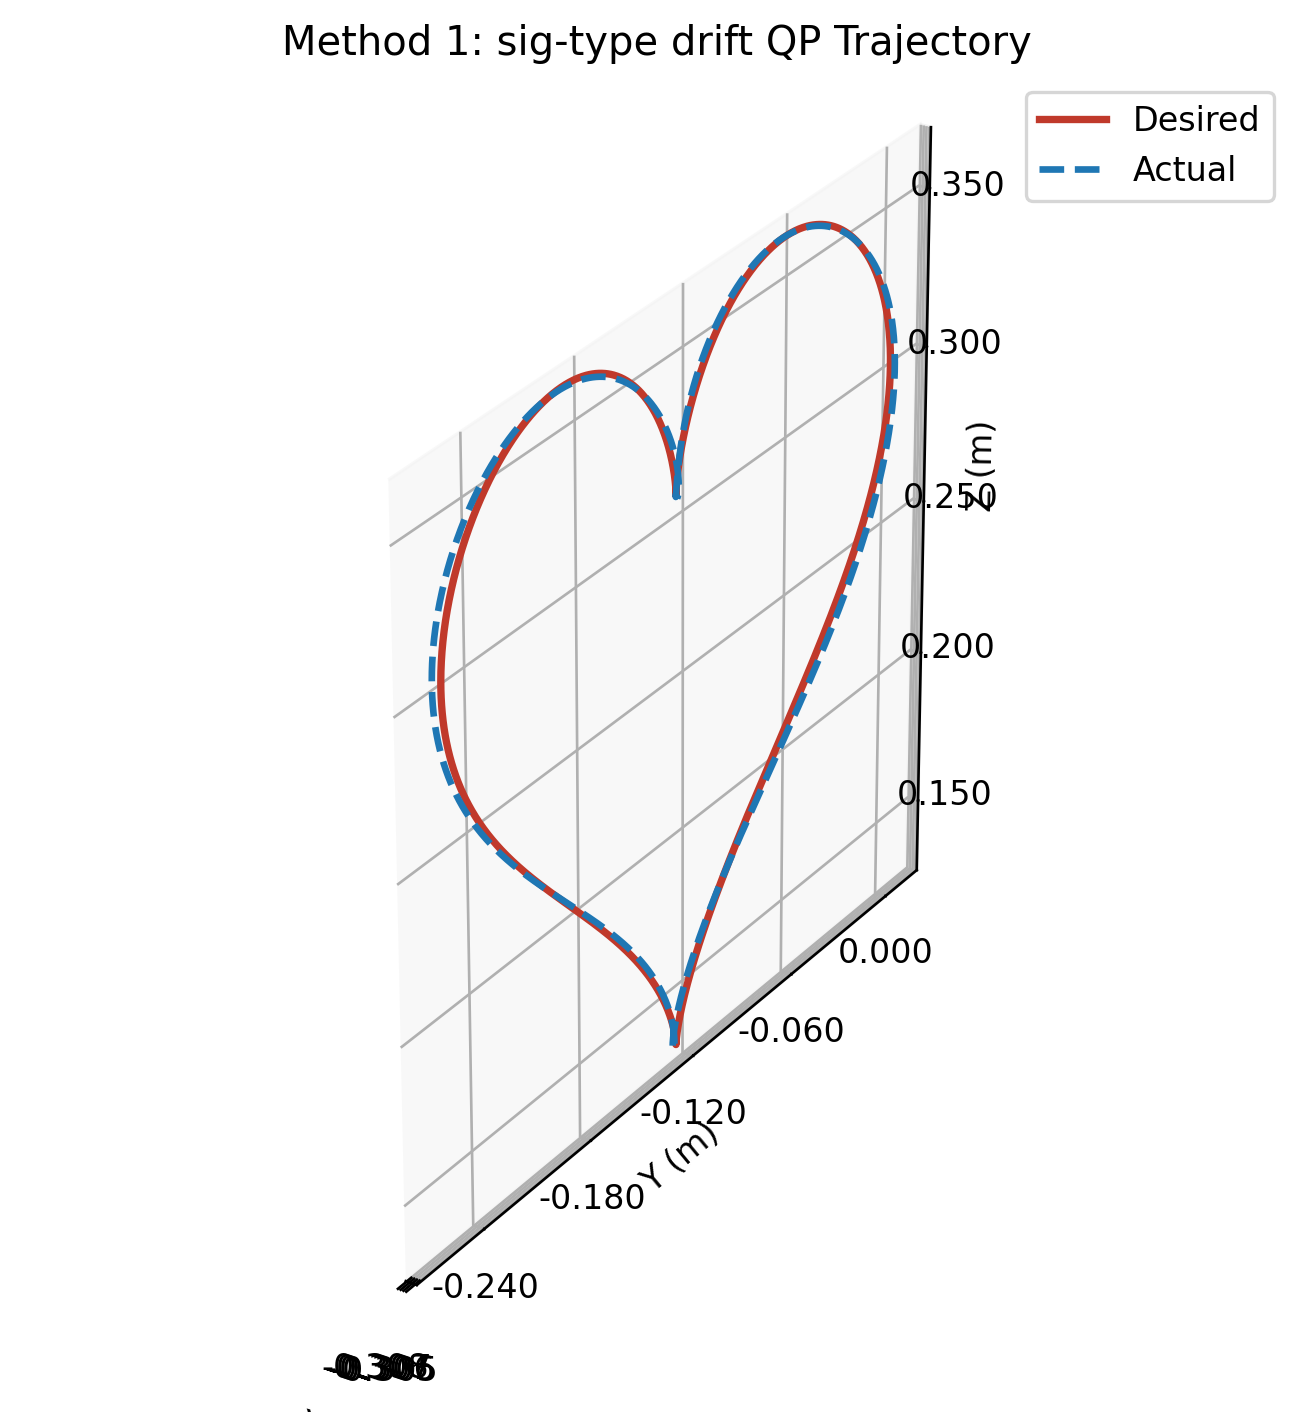
\includegraphics[width=0.68\linewidth]{method1_live_trajectory.png}
  \caption{Simulator based real time trajectory of the original \methodone{}.}
\end{figure}

\begin{figure}[H]
  \centering
  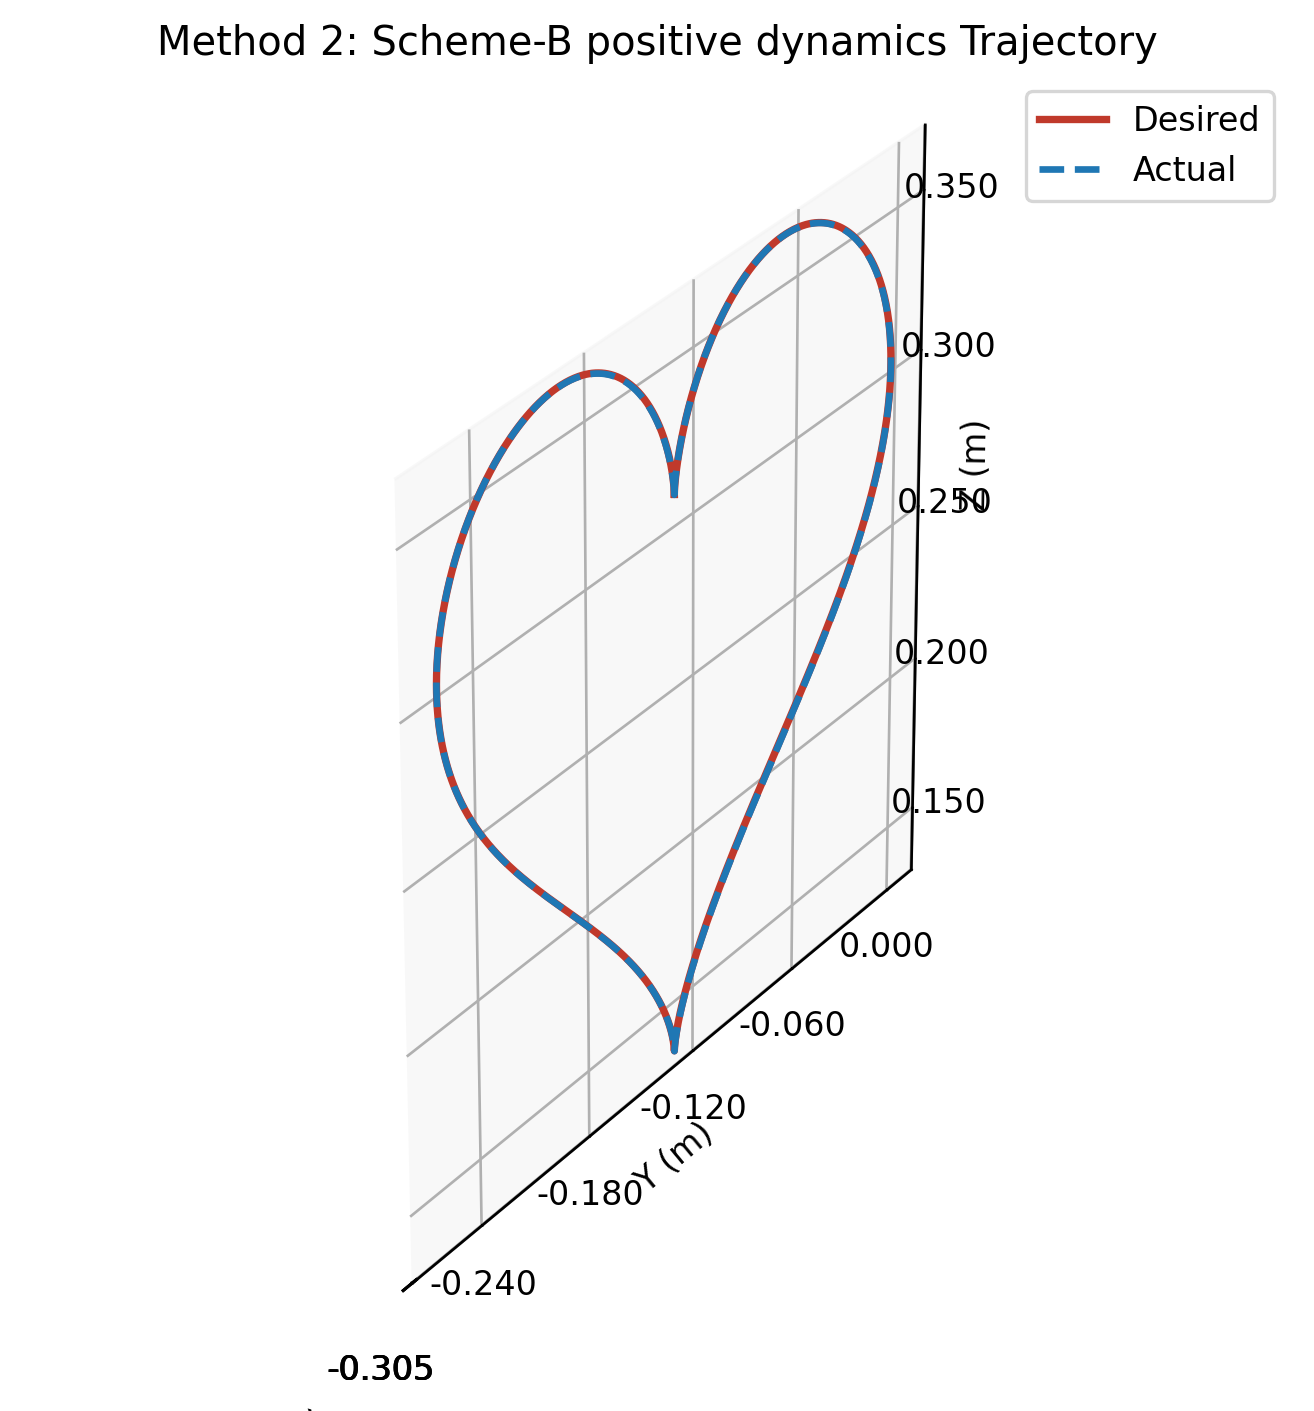
\includegraphics[width=0.68\linewidth]{method2_live_trajectory.png}
  \caption{Simulator based real time trajectory of the original \methodtwo{}.}
\end{figure}

\begin{figure}[H]
  \centering
  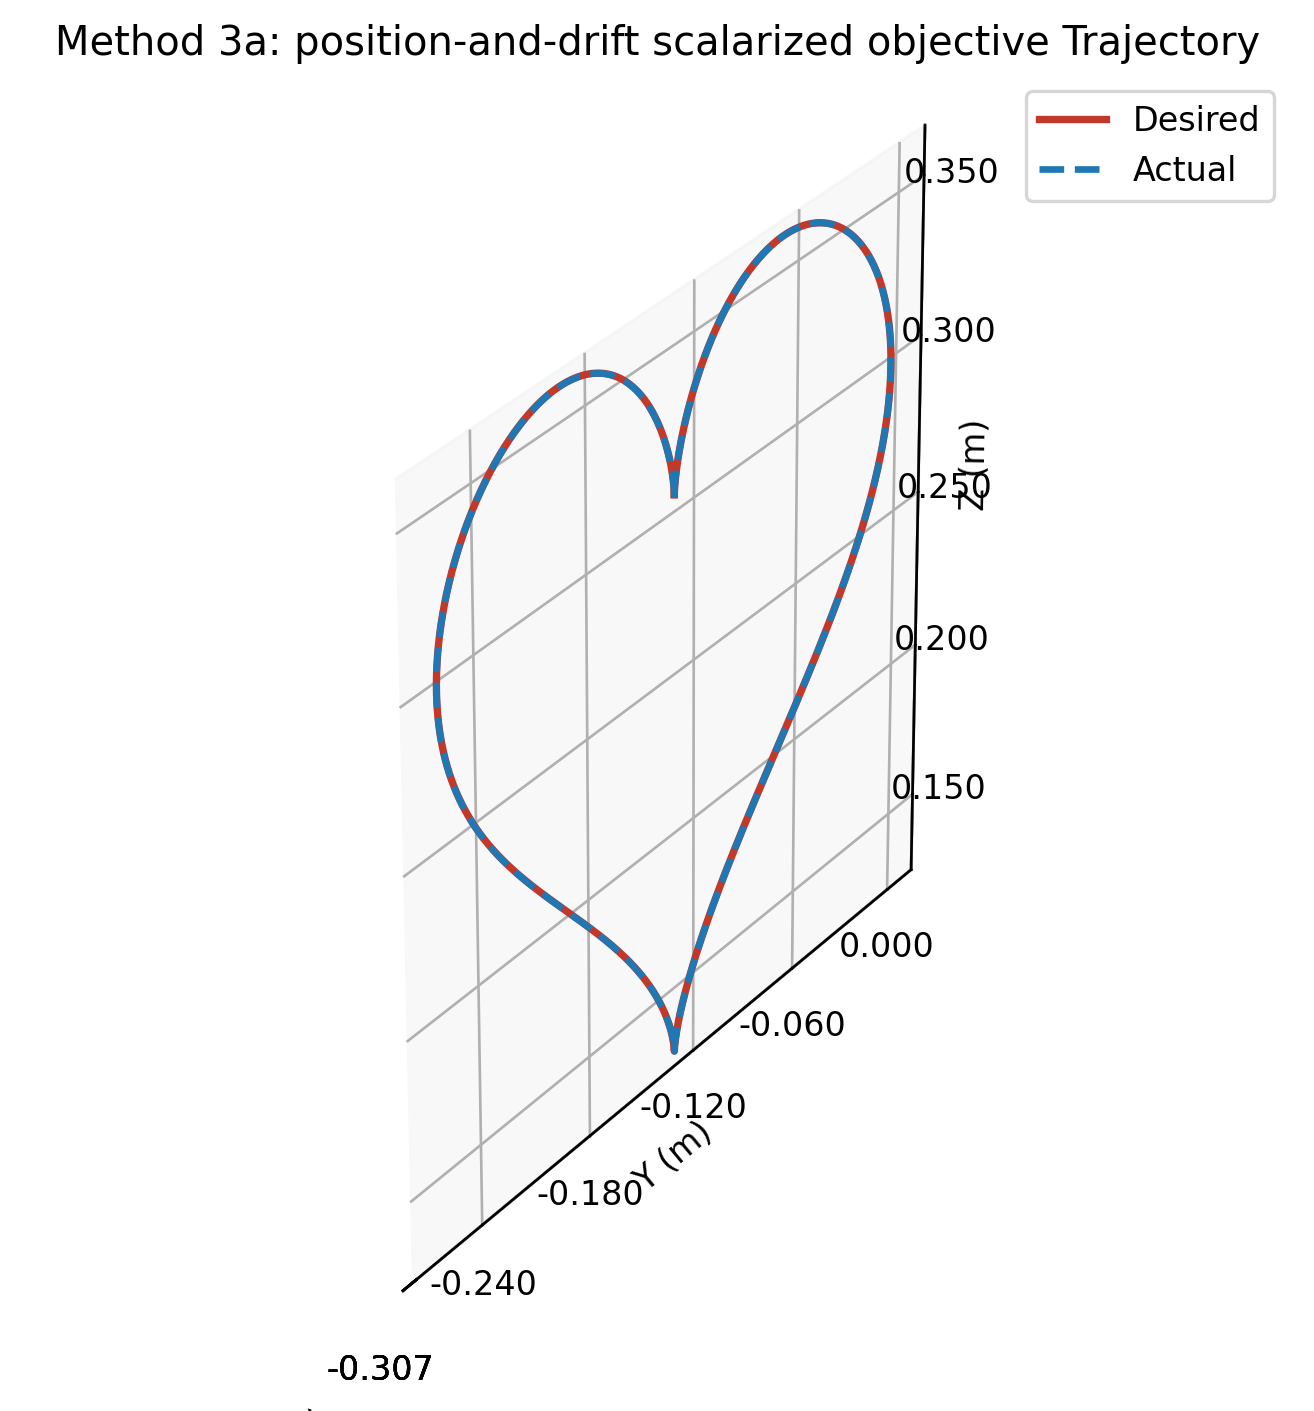
\includegraphics[width=0.68\linewidth]{method3a_live_trajectory.png}
  \caption{Simulator based real time trajectory of the original \methodthree{}.}
\end{figure}

\begin{figure}[H]
  \centering
  
\includegraphics[width=0.76\linewidth]{method3c_position_and_drift_lccznn_live_joint_drift.png}
  \caption{Simulator based real time joint drift history of \methodthreelcc{}.}
\end{figure}

\begin{figure}[H]
  \centering
  
\includegraphics[width=0.68\linewidth]{method3a_position_and_drift_pcg_live_trajectory.png}
  \caption{Representative simulator based real time trajectory of \methodthreepcg{}.}
\end{figure}

\begin{figure}[H]
  \centering
  
\includegraphics[width=0.76\linewidth]{method3a_position_and_drift_pcg_live_inner_iterations.png}
  \caption{Inner iteration count history of \methodthreepcg{}.}
\end{figure}

\begin{figure}[H]
  \centering
  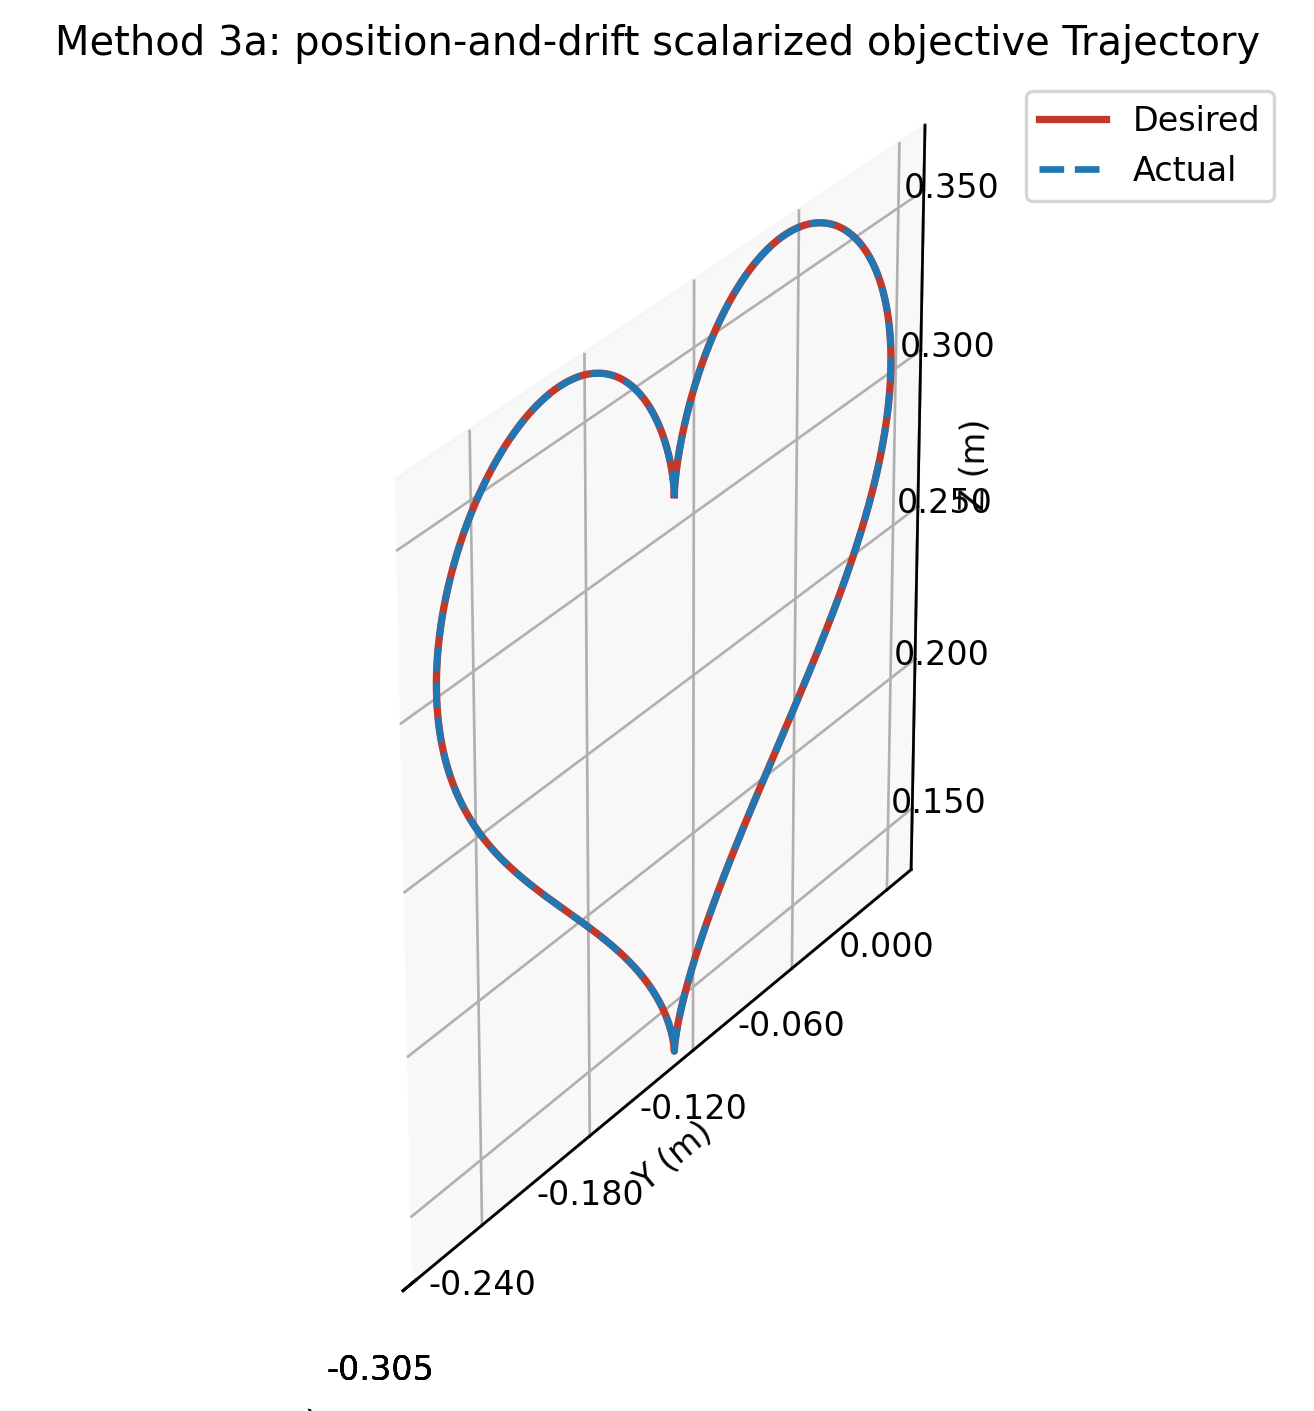
\includegraphics[width=0.70\linewidth]{method3a_live20_trajectory.png}
  \caption{Extended \SI{20}{\second} simulator based real time trajectory of the original \methodthree{}.}
\end{figure}


\end{document}
